\documentclass[]{interact}
% Use Latin Modern fonts
\usepackage{lmodern}
\usepackage{float}
\usepackage{graphicx}
% Include algorithm2e for algorithm environment
\usepackage[ruled,vlined]{algorithm2e}
% To incorporate .eps illustrations using PDFLaTeX
\usepackage{epstopdf}
% Support for small, `sub' figures and tables
\usepackage[caption=false]{subfig}
% Citation support using natbib.sty
\usepackage[numbers,sort&compress]{natbib}
% Citation support using natbib.sty
\bibpunct[, ]{[}{]}{,}{n}{,}{,}
% Bibliography support using natbib.sty
\renewcommand\bibfont{\fontsize{10}{12}\selectfont}
% @ becomes a letter
\makeatletter
% Suppress spaces between citations using natbib.sty
\def\NAT@def@citea{\def\@citea{\NAT@separator}}
% @ becomes a symbol again
\makeatother
% Theorem-like structures provided by amsthm.sty
\theoremstyle{plain}
\newtheorem{theorem}{Theorem}[section]
\newtheorem{lemma}[theorem]{Lemma}
\newtheorem{corollary}[theorem]{Corollary}
\newtheorem{proposition}[theorem]{Proposition}
% 
\theoremstyle{definition}
\newtheorem{definition}[theorem]{Definition}
\newtheorem{example}[theorem]{Example}
%
\theoremstyle{remark}
\newtheorem{remark}{Remark}
\newtheorem{notation}{Notation}


\begin{document}


\articletype{RESEARCH ARTICLE}

\title{Cost-Optimized Data Partitioning for Parallel Sorting on Heterogeneous Distributed Systems using Mixed Integer Programming}

\author{
\name{Joeniño Cainday and Dr. Junar Landicho}
% TODO: thanks is on the template
% \thanks{CONTACT Joeniño Cainday. Email: caindayjoeninyo@gmail.com}
\affil{Department of Computer Science, University of Science and Technology of Southern Philippines, Cagayan De Oro City, Philippines}
}

\maketitle

\begin{abstract}
This research addresses the optimization of data partitioning for parallel computations in heterogeneous distributed systems, with the dual objective of minimizing financial expenditure and execution time. We develop a Mixed Integer Programming (MIP) model that incorporates critical system constraints including CPU speed, memory capacity, memory latency, network latency, and budget limitations. Our model replaces the heuristic partitioning phase of a parallel quicksort algorithm, which serves as our performance benchmark. Utilizing synthetic datasets representing both workload and node specifications, our simulations focus on pre-execution data partitioning decisions. The goal is to provide a framework for financial and time optimization within cloud computing environments, where efficient resource allocation and budget management are essential. Results demonstrate the effectiveness of our MIP-based approach in achieving improved load distribution and reduced runtime compared to traditional heuristics.
\end{abstract}

\begin{keywords}
Data Partitioning; Mixed Integer Programming; Heterogeneous Distributed Systems; Budget Constraints; Makespan Minimization
\end{keywords}

\section{Introduction}

The widespread adoption of cloud computing and serverless architectures has increased the importance of efficient resource allocation in distributed systems. This research addresses the challenge of statically partitioning data across heterogeneous computing environments, where nodes vary in processing speed, memory capacity, network latency, and monetary implications.

We formulate data partitioning as an NP-hard combinatorial optimization problem aimed at minimizing execution time (makespan) while adhering to defined constraints. Our approach replaces traditional heuristic-based partitioning in parallel sorting algorithms with a novel Mixed Integer Programming (MIP) model designed to capture comprehensive system constraints for more balanced, resource-aware data distributions.

\subsection{Background and Motivation}

Distributed computing enables parallel processing of large-scale datasets across multiple nodes. However, in heterogeneous systems with diverse computational capabilities, simplistic data partitioning strategies often result in load imbalances and inefficient resource utilization [1]. Common approaches like uniform distribution or partitioning based solely on heuristics typically fail to consider system compositions in cloud environments.

Cloud computing introduces new complexities to data partitioning. These environments offer flexibility with pay-as-you-go pricing models where computing resources are available on demand [5]. This necessitates re-evaluating traditional partitioning methodologies to explicitly consider economic factors alongside performance metrics. Effective strategies must balance high performance with budget limitations—minimizing both computational time and overall expenditure for cloud resource utilization. 

While Monga and Lodhi [53] demonstrated benefits of heterogeneity-aware allocation, their model primarily considered CPU speed alone. Our work introduces a more sophisticated MIP-based model that integrates multiple system attributes to achieve globally optimized data distributions, providing a more realistic and budget-conscious approach to optimized data processing.


\subsection{Cost Considerations in Heterogeneous Distributed Systems}

This paper specifically addresses statically partitioning large datasets before executing parallel sorting across simulated heterogeneous environments. Our primary objective is to minimize the overall execution time (makespan) while ensuring we satisfy the defined constraints. As a secondary objective, we aim to identify the most budget-effective solution with an equivalent makespan, using a lexicographic optimization approach. 

In this context, cost refers to the pricing of cloud compute nodes. While higher-priced instances often imply better performance, this is not guaranteed, as pricing and performance can vary across vendors. Each simulated node has synthetic attributes including processing speed, memory capacity, network characteristics, and pricing models inspired by real cloud offerings, reflecting typical variations in heterogeneous cloud deployments.

Allocating data across heterogeneous resources inherently involves performance-cost tradeoffs [48]. As highlighted in previous research, balancing processing time with financial implications when assigning datasets to different machines is critical. Effective data partitioning can significantly reduce both runtime and monetary cost, while suboptimal partitioning leads to inflated expenses or resource limitations like memory overflows. Our controlled synthetic environment enables repeatable experiments independent of real-world cloud variability.

MIP provides a powerful mathematical framework for complex optimization problems involving both discrete and continuous decision variables subject to linear constraints [8]. This capability makes MIP well-suited for modeling cost-aware data partitioning in heterogeneous systems:

\begin{itemize}
    \item Discrete variables represent partitioning decisions (assigning specific data blocks to particular nodes)
    \item Continuous variables model resource utilization levels and associated costs
    \item The objective function represents total financial expenditure
    \item Constraints reflect resource limitations and system characteristics
\end{itemize}

Through this approach, MIP effectively finds optimal or near-optimal partitioning strategies that minimize expenditure while satisfying performance requirements.

\subsection{Research Contributions}

This paper contributes the following:
\begin{enumerate}
    \item A MIP formulation for initial data partitioning in parallel quicksort on heterogeneous systems;
    \item An integration of the MIP model into an existing heterogeneous sorting framework;
    \item A performance evaluation using synthetic datasets with extended metrics;
    \item A reproducible experimental setup and discussion of directions for future work.
\end{enumerate}


\section{Related Work}
\label{sec:related_work}
Heterogeneous scheduling and data allocation have been studied in various contexts. [48] considered dataset allocation across geo-distributed clouds with two objectives (processing time and cost) [48]. They formulated a linear program to place data blocks on VMs to minimize weighted sum of time and cost, demonstrating Pareto trade-offs. Similarly, [49] used an integer linear program for data assignment in a hybrid heterogeneous processing environment. These works focus on resource assignment rather than within-job data partitioning, but they highlight the utility of mathematical programming for cloud costs.

Classic scheduling theory demonstrates that even simple load-balancing on unrelated machines is NP-hard [50]. For instance, scheduling jobs to minimize makespan in  admits a 2-approximation algorithm but cannot be solved optimally in polynomial time beyond trivial cases [50]. This complexity motivates the treatment of cost-aware data partitioning as a combinatorial optimization problem, which is closely related to  but with additional cost considerations. This can be extended to multi-objective formulations (e.g., cost and makespan), though even the single-objective version is NP-hard, reducible to scheduling on unrelated parallel machines [50].

In the domain of parallel sorting, many algorithms assume a homogeneous machine model. For instance, Parallel Sorting by Regular Sampling (PSRS) chooses pivots to create equally-sized partitions [51], and typical benchmarks use randomly-generated data with uniform or other distributions [51]. These benchmarks (e.g. uniform 32-bit integer inputs) guide our synthetic data choices. However, PSRS and related methods do not account for cost or heterogeneous speeds.

In big-data systems like Spark, dynamic partitioning and scheduling algorithms have been proposed. [52], for example, developed a dynamic partitioning strategy for intermediate Spark data to mitigate skew, and a greedy scheduling method that considers node speed [52]. They find that balanced partitioning significantly lowers completion time [52]. Our work differs by focusing on static initial partitioning with explicit cost metrics, rather than in-job rebalancing. To the best of our knowledge, prior work has not explicitly applied MIP to cost-aware static data partitioning in heterogeneous cloud sort workloads.

We build upon the model proposed by Monga and Lodhi~\cite{monga2020heterogeneous}, which partitions data across heterogeneous nodes based on CPU performance to balance load during parallel sorting. However, their approach does not consider critical real-world factors such as network latency or resource cost—key limitations in cloud and serverless settings. Moreover, their method performs initial local sorting and sampling before defining data ranges, which can lead to uneven memory usage and load imbalance during the redistribution phase.




% This section presents our approach combining Mixed Integer Programming (MIP) for optimal data partitioning with the parallel Quicksort algorithm proposed by Monga and Lodhi [53].

\section{Problem Formulation}

We now formalize the partitioning problem based on the system characteristics introduced in Section 1.3. To ensure full control over system parameters and facilitate reproducibility, we operate within a synthetic environment. Each node is defined by parameters such as processing speed, memory capacity, network latency, bandwidth, and cost, inspired by real-world cloud configurations (e.g., AWS, GCP). This abstraction enables rigorous evaluation of partitioning strategies without relying on live infrastructure.

\subsection{System Model}

We partition the dataset into contiguous blocks of size $d$, assigning each block to a unique node. Consider a heterogeneous cluster with $N$ nodes, where each node $i$ is characterized by the following parameters:

\begin{itemize}
    \item $d_i$: Assigned data volume (in units of $d$)
    \item $r_i$: Processing rate (in $d/t$ — data units per time unit)
    \item $m_i$: Maximum data volume the node can handle at once (in units of $d$)
    \item $\ell_i$: Network latency (in time units $t$)
    \item $b_i$: Network bandwidth (in $d/t$ — data units per time unit)
    \item $u_i$: Usage billing rate (in $c/t$ — cost units per time unit)
\end{itemize}

The units above are illustrative and can be adapted depending on context. For instance, processing speed $r$ may be measured in records/ms, memory $m$ in megabytes (MB), and cost $u$ in USD/hour. In this work, we use normalized or synthetic units to model relative performance and cost differences between nodes, without binding the system to a specific infrastructure or currency.

\subsection{Derived Parameters}
We derive additional parameters from the node characteristics to facilitate the MIP formulation:

\subsubsection{Processing Time}
\begin{equation}
    x_i = \frac{d_i}{r_i}
\end{equation}
where $x_i$ is the time required by node $i$ to process its assigned data volume $d_i$.

\subsubsection{Transfer Time}
\begin{equation}
    y_i = \ell_i + \frac{d_i}{b_i}
\end{equation}
where $y_i$ is the communication overhead for node $i$, computed from latency $\ell_i$ and bandwidth $b_i$.

\subsubsection{Total Cost}
\begin{equation}
    w = \sum_{i=1}^N u_i \cdot x_i
\end{equation}
where $w$ denotes the cumulative cost of utilizing all selected nodes.

\subsection{Optimization Objectives}
The primary objective of our MIP model is to minimize the total execution time (makespan) of the parallel sorting process. This ensures that the overall completion time is minimized, taking into account both computation and communication overheads. Formally, the primary objective is defined as:
\begin{equation}
    \min z = \max_{i=1}^N (x_i + y_i)
\end{equation}
where $z$ represents the maximum time taken by any node $i$ to complete its assigned data processing and communication tasks. This formulation captures the makespan of the entire parallel sorting operation, ensuring that the slowest node determines the overall completion time. In addition to minimizing makespan, we aim to choose the most cost-effective solution among equivalent combinations. To achieve this, we introduce a secondary objective that minimizes the total financial expenditure. This is incorporated into the model using a lexicographic optimization approach:
\begin{equation}
    \min \ z + \varepsilon \cdot w
\end{equation}
In this formulation, $w$ represents the cumulative cost of utilizing the selected nodes, and $\varepsilon$ is set to a negligible value (e.g., $10^{-6}$) to prioritize makespan minimization while breaking ties in favor of cost efficiency. This approach ensures that among solutions with equivalent makespan, the one with the lowest cost is selected.

\subsection{Constraint Definitions}

The proposed MIP model is subject to several constraints that reflect system limitations and ensure a feasible allocation of data across nodes. These constraints incorporate resource boundaries (e.g., memory and budget), performance considerations (e.g., makespan), and completeness of the partitioning scheme.

\subsubsection{Makespan Constraint}
\begin{equation}
    z \geq \frac{d_i}{r_i} + \ell_i + \frac{d_i}{b_i} \quad \forall i \in \{1, \ldots, N\}
\end{equation}
This constraint ensures that the total execution time, represented by the variable $z$, is at least as large as the time taken by any individual node $i$ to both process its assigned data and transfer it to the next stage. It combines computation time $\frac{d_i}{r_i}$ with communication latency $\ell_i$ and data transfer time $\frac{d_i}{b_i}$.

\subsubsection{Memory Constraint}
\begin{equation}
    d_i \leq m_i \quad \forall i \in \{1, \ldots, N\}
\end{equation}
Each node has a limited memory capacity $m_i$, and this constraint ensures that the volume of data $d_i$ assigned to node $i$ does not exceed its available memory.

\subsubsection{Coverage Constraint}
\begin{equation}
    \sum_{i=1}^{N} d_i = D
\end{equation}
This constraint enforces full data allocation: the entire dataset of size $D$ must be partitioned and distributed among the $N$ available nodes without omission or duplication.

\subsubsection{Non-negativity Constraint}
\begin{equation}
    d_i \geq 0 \quad \forall i \in \{1, \ldots, N\}
\end{equation}
This standard constraint ensures that each node receives a non-negative volume of data, reflecting the physical impossibility of assigning negative quantities.


\subsubsection{Budget Constraint (Optional)}
\begin{equation}
    0 \leq \sum_{i=1}^{N} u_i \cdot d_i \leq B
\end{equation}
In addition to node-specific parameters, we optionally define a user-defined input $B$, representing the maximum allowable expenditure. This parameter must be a non-negative number, with a default value of $0$. Including this constraint models scenarios where financial limitations must be respected.











\section{Heterogeneous PSRS (Baseline Algorithm)}

This is the model of Monga and Lodhi [53] which we will use as a baseline. The algorithm is designed to sort a list of items using multiple workers, each with different speeds. The main steps of the algorithm are as follows:

\begin{algorithm}[H]
\caption{Heterogeneous PSRS (Baseline Algorithm)}
\SetKwInput{KwInput}{Inputs}
\KwInput{
    \begin{itemize}
        \item $data$: Input data to be sorted
        \item $n$: Total number of data items
        \item $p$: Number of processors
        \item $perf[0 \dots p-1]$: Relative performance of each processor
    \end{itemize}
}
\SetKwInput{KwOutput}{Output}
\KwOutput{
    \begin{itemize}
        \item Sorted data
    \end{itemize}
}

\textbf{Phase 1: Local Sorting and Sampling} \\
\For{each processor $i$}{
    $size_i = \frac{n \cdot perf[i]}{\sum perf}$ \\
    Assign $size_i$ items to processor $i$ \\
    Processor $i$ performs sequential quicksort on its local data \\
    Select $L = (p - 1) \cdot perf[i]$ samples from local sorted data \\
    Send samples to the designated coordinator
}

\textbf{Phase 2: Pivot Selection} \\
Designated coordinator gathers and sorts all samples \\
Selects $p - 1$ global pivots and broadcasts them to all processors

\textbf{Phase 3: Data Redistribution} \\
\For{each processor}{
    Partition local data using global pivots \\
    Send partitioned data to corresponding processors \\
    Retain the portion corresponding to its final range
}

\textbf{Phase 4: Final Sorting and Merge} \\
Each processor sorts its final local data \\
Coordinator concatenates all sorted segments for final output
\end{algorithm}

\subsection{Limitations}

While the Heterogeneous PSRS algorithm by Monga and Lodhi~\cite{monga2020heterogeneous} offers an effective strategy for distributing sorting tasks across processors of varying speeds, it introduces several inefficiencies. The algorithm performs local sorting before establishing the global data partitions, which can result in skewed data distributions during the redistribution phase. This may lead to certain processors receiving significantly larger portions of data, causing load imbalance and increased memory consumption. Furthermore, the algorithm does not account for communication cost or network latency, which are vital considerations in distributed and cloud-based environments. These shortcomings motivate the need for a more adaptive approach that considers both performance and cost constraints when assigning data ranges.






\section{MIP-Guided Sorting (Proposed Algorithm)}

We propose a modified algorithm that replaces the sampling and redistribution stages with a Mixed Integer Programming (MIP) formulation that statically partitions the global key range across heterogeneous distributed nodes.

\subsection{Bucket Assignment}

Given the total dataset size $D$ and a heterogeneous set of $N$ nodes with parameters $(r_i, m_i, \ell_i, b_i, u_i)$, we solve the MIP formulation (Section~\ref{sec:methodology}) to compute optimal partition sizes $d_i$ such that:

\begin{itemize}
    \item Processing time is balanced according to each node's capability
    \item Communication and processing costs are minimized
    \item Constraints on memory, load, and budget are respected
\end{itemize}

Once $d_i$ values are determined, each node is assigned a fixed key range. For example (illustrative only):

\begin{center}
\begin{tabular}{|p{4cm}|p{5cm}|p{4cm}|}
\hline
\textbf{Worker} & \textbf{Percentage of Total Data} & \textbf{Assigned Range} \\
\hline
A (4x speed) & 50\% & [0, 49] \\
\hline
B (3x speed) & 30\% & [50, 79] \\
\hline
C (2x speed) & 20\% & [80, 100] \\
\hline
\end{tabular}
\end{center}

\subsection{Proposed Algorithm}

\begin{algorithm}[H]
\caption{MIP-Guided Bucket-Quicksort Hybrid (Proposed Algorithm)}

\SetKwInput{KwInput}{Inputs}
\KwInput{
    \begin{itemize}
        \item $D$: Total dataset
        \item $N$: Number of nodes
        \item $r_i$: Processing rate of node $i$
        \item $m_i$: Memory capacity of node $i$
        \item $b_i$: Network bandwidth of node $i$
        \item $\ell_i$: Network latency of node $i$
        \item $u_i$: Usage cost rate of node $i$
    \end{itemize}
}

\SetKwInput{KwOutput}{Output}
\KwOutput{
    \begin{itemize}
        \item Sorted data
    \end{itemize}
}

\textbf{Phase 1: Static Partitioning via MIP} \\
Solve MIP to determine partition sizes $d_i$ for each node \\
Assign key ranges to nodes based on $d_i$ and global key distribution

\textbf{Phase 2: Data Distribution} \\
\For{each item $x$ in $D$}{
    Route $x$ to processor $i$ such that $x$ lies in $i$'s assigned key range
}

\textbf{Phase 3: Local Sorting} \\
\For{each processor $i$}{
    Sort received data using sequential quicksort
}

\textbf{Phase 4: Final Merge (Optional)} \\
Concatenate sorted outputs from all nodes

\end{algorithm}

\subsection{Distribution Strategies}

\subsubsection{Option A: Centralized Bucketing (Low Latency, High Memory)}
\begin{itemize}
    \item A single coordinator receives all input data and routes items to target nodes
    \item Requires $2 \times$ dataset size in memory
    \item Low latency and simple coordination, but limited scalability
\end{itemize}

\subsubsection{Option B: Asynchronous Routing (Low Memory, High Latency)}
\begin{itemize}
    \item Each item is routed asynchronously to its responsible node
    \item Lower memory footprint, suited for streaming or distributed sources
    \item May incur higher latency due to decentralized routing
    \item Increases billing costs due to more frequent node usage
\end{itemize}








\section{Theoretical Complexity Analysis}

A rigorous complexity analysis highlights the theoretical advantages of our MIP-guided approach over the baseline PSRS algorithm, particularly in heterogeneous distributed nodes.

\subsection{Baseline Algorithm}

\subsubsection{Time Complexity}
The original Heterogeneous PSRS algorithm involves four distinct phases, each contributing to the overall time complexity:

\paragraph{Phase 1: Local Sorting and Sampling} 
Each of the $p$ processors sorts its local data of size $O(n/p)$ on average, taking $O\left(\frac{n}{p} \log \frac{n}{p}\right)$ time using quicksort. Sampling takes $O(p)$ time per processor. The communication of samples to the coordinator takes $O(p^2)$ in the worst case if all processors send their $O(p)$ samples sequentially. Thus, this phase has an average time complexity of $O\left(\frac{n}{p} \log \frac{n}{p} + p^2\right)$.

\paragraph{Phase 2: Pivot Selection. }
The coordinator sorts $O(p^2)$ samples, which takes $O(p^2 \log p^2) = O(p^2 \log p)$ time. Broadcasting the $p - 1$ pivots to all $p$ processors takes $O(p)$ time in parallel or $O(p^2)$ sequentially.

\paragraph{Phase 3: Data Redistribution} Each processor partitions its $O(n/p)$ local data using $p - 1$ pivots, which takes $O(n/p \cdot p) = O(n)$ in the worst case if the pivots are poorly chosen. The redistribution of data among processors can take up to $O(n)$ in the worst-case scenario where one processor receives almost all the data.

\paragraph{Phase 4: Final Sorting and Merge} Each processor sorts its received data, which can be up to $O(n)$ in the worst case, leading to $O(n \log n)$ for a single processor if load balancing is poor. The coordinator then merges the $p$ sorted segments, which takes $O(n)$ time.

\paragraph{Overall Complexity} Combining these phases, the average-case time complexity of the original PSRS algorithm is dominated by the local sorting and pivot selection, yielding $O\left(\frac{n}{p} \log \frac{n}{p} + p^2 \log p + n\right)$. Under ideal load balancing, this simplifies to $O\left(\frac{n \log n}{p} + p^2 \log p\right)$. The worst-case time complexity, particularly due to potential imbalances in data redistribution, can reach $O(n \log n)$ if one processor ends up with most of the data, or even $O(n^2/p)$ if local sorting on an imbalanced partition degrades to quadratic time.


\subsubsection{Space Complexity}
For space complexity, the PSRS algorithm requires local storage for each processor to store its assigned data, which is $O(n/p)$ on average. Sampling generates $O(p)$ samples per processor, and the coordinator stores $O(p^2)$ samples. During data redistribution, processors might need temporary buffers to hold data being sent or received, potentially up to $O(n/p)$ in size per processor. Each processor holds a sorted segment of approximately $O(n/p)$. The total space complexity of the PSRS algorithm is $O(n)$ as the total data is partitioned and stored across the processors. The coordinator requires additional space for the samples, $O(p^2)$.

\subsection{Proposed Algorithm}
For the MIP-guided algorithm, the process is significantly streamlined. 

\subsubsection{Time Complexity}
\paragraph{Phase 1: Static partitioning via MIP}
This is solved once as a precomputation step. The complexity of solving a general MIP is NP-hard. However, for a fixed number of nodes $N$, the complexity can be bounded by a polynomial function of the input size, which in our case relates to the number of nodes and the complexity of the constraints. Assuming an efficient solver, and considering the number of variables (proportional to $N$) and constraints (also proportional to $N$), a loose upper bound can be considered around $O(N^k)$ for some constant $k$, potentially up to $O(N^3)$ for simpler formulations or higher for more complex ones. This is a one-time overhead.

\paragraph{Phase 2: Data Distribution} For Option A (Centralized Bucketing), the coordinator processes each of the $n$ items once to route it, taking $O(n)$ time. For Option B (Asynchronous Routing), each of the $n$ items is routed directly to a processor. Assuming the routing decision is constant time, this phase takes $O(n)$ time in total, potentially distributed across the network.

\paragraph{Phase 3: Local Sorting} Each of the $N$ processors sorts its assigned data of size $d_i$. Since the MIP aims to balance the load based on processing rates, we expect $d_i \approx O(n/N)$. Thus, the local sorting on each processor takes approximately $O\left(\frac{n}{N} \log \frac{n}{N}\right)$. Executed in parallel, the time for this phase is $O\left(\frac{n}{N} \log \frac{n}{N}\right)$.

\paragraph{Phase 4: Final Merge (optional)}. If a final merged output is required, the coordinator concatenates the $N$ sorted segments, taking $O(n)$ time. This step can be avoided if the output is acceptable as a set of distributed sorted partitions.

\paragraph{Overall Complexity} Therefore, the overall time complexity of the MIP-guided algorithm, after the initial MIP solving, is dominated by the data distribution and local sorting phases, resulting in an average and worst-case time complexity of $O(N^k + n + \frac{n}{N} \log \frac{n}{N})$. If $N$ is significantly smaller than $n$, this simplifies to $O(n + \frac{n}{N} \log \frac{n}{N})$. The one-time MIP solving overhead $O(N^k)$ becomes negligible for large datasets processed multiple times.

\subsubsection{Space Complexity}

For the MIP-guided algorithm, partition storage requires each of the $N$ nodes to store its assigned partition of size $d_i$, with $\sum d_i = n$. Thus, the total storage for the data is $O(n)$. For data distribution, 

\paragraph{Option A: (Centralized Bucketing)} Temporarily holds the entire dataset for routing, requiring $O(n)$ additional space, leading to a total of $O(2n)$ peak memory usage at the coordinator. 

\paragraph{Option B: (Asynchronous Routing)} Routes each item individually, minimizing the need for a central buffer. The memory footprint remains $O(n)$ distributed across the nodes. Local sorting requires each processor to sort its local partition $d_i$ in-place or requires $O(d_i)$ auxiliary space, which is within the $O(n)$ total. The space required for storing the MIP model and its solution is dependent on the solver and the complexity of the formulation but is typically much smaller than the dataset size $n$, especially for a fixed number of nodes $N$.



\subsection{Complexity Comparison}


In this section, we formally analyze and compare the time complexity of the baseline PSRS algorithm and the proposed MIP-guided algorithm. The analysis emphasizes both average-case behavior and worst-case scenarios under heterogeneous processing environments.

\subsubsection{Baseline Algorithm}

The PSRS algorithm executes in four distinct phases: local sorting and sampling, pivot selection, data redistribution, and final sorting or merging. The overall time complexity is characterized as follows:

\begin{equation}
    \mathcal{O}\left(\frac{n}{p} \log \frac{n}{p} + p^2 \log p + n\right)
\end{equation}

Under ideal load balancing and efficient communication, this simplifies to:

\begin{equation}
    \mathcal{O}\left(\frac{n \log n}{p} + p^2 \log p\right)
\end{equation}

However, due to dynamic pivot selection and possible load imbalance, the worst-case time complexity may degrade to:

\begin{equation}
    \mathcal{O}(n \log n)
\end{equation}

This degradation arises when a significant portion of data is allocated to a single processor due to poor pivot selection.

\subsubsection{Proposed Algorithm}

The MIP-guided algorithm separates the partitioning step as a one-time optimization via a Mixed Integer Programming formulation. After solving the MIP, the data is distributed based on a precomputed partitioning strategy that accounts for processor heterogeneity. The total time complexity is expressed as:

\begin{equation}
    \mathcal{O}\left(N^k + n + \frac{n}{N} \log \frac{n}{N}\right)
\end{equation}

Here, $N$ is the number of processors and $k$ is a constant that depends on the complexity of the MIP formulation. This overhead is incurred once and amortized over multiple executions. The dominant runtime costs after MIP solving are data distribution and local sorting.



\subsubsection{Formal Complexity Comparison}

\begin{table}[H]\
\centering
\begin{tabular}{|p{6.6cm}|p{6.6cm}|}
\hline
\textbf{Algorithm} & \textbf{Time Complexity} \\
\hline
PSRS (Best/Average) & $O\left(\dfrac{n \log n}{p} + p^2 \log p\right)$ \\
\hline
PSRS (Worst-case) & $O(n \log n)$ \\
\hline
MIP-Guided & $O\left(N^k + n + \dfrac{n}{N} \log \dfrac{n}{N}\right)$ \\
\hline
\end{tabular}
\end{table}


\begin{table}[H]
\centering
\begin{tabular}{|p{6.6cm}|p{6.6cm}|}
\hline
\textbf{Algorithm} & \textbf{Space Complexity} \\
\hline
PSRS (Baseline) & $O(n)$ total; includes buffers for redistribution and samples. \\
\hline
MIP-Guided (Centralized Bucketing) & $O(2n)$; requires double memory at the coordinator for routing. \\
\hline
MIP-Guided (Asynchronous Routing) & $O(n)$; distributed memory usage with minimal central buffer. \\
\hline
\end{tabular}
\end{table}

\begin{figure}[h] % 'h' means 'here'
    \centering
    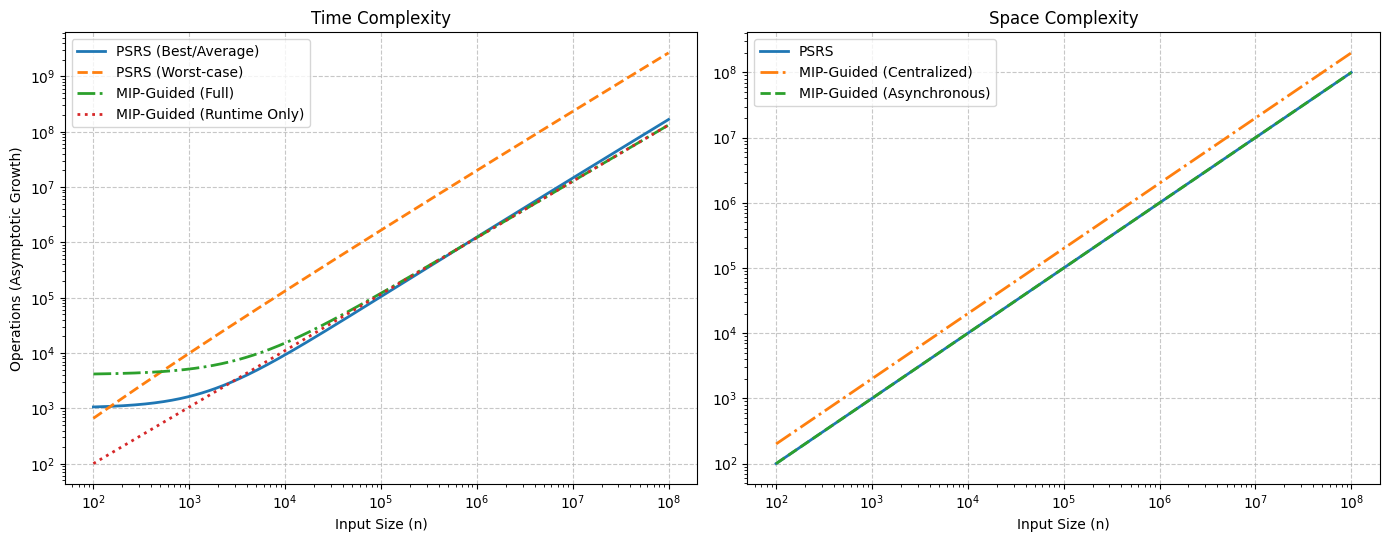
\includegraphics[width=1\textwidth]{graph-complexity.png}
    \label{fig:example}
\end{figure}


\subsubsection{Performance Factors Comparison}

\begin{table}[H]
\begin{tabular}{|p{3cm}|p{5cm}|p{5cm}|}
\hline
\textbf{Aspect} & \textbf{PSRS} & \textbf{MIP-Guided} \\
\hline
Load Balancing & Data-dependent and dynamic, prone to imbalance & Statistically balanced using processor profiles \\
\hline
Synchronization & Multiple barriers: sampling, pivoting, merging & Minimal, only at merge (if needed) \\
\hline
Communication Overhead & $O(p^2)$ (samples), $O(n)$ (data) & $O(n)$ (initial only) \\
\hline
Preprocessing & None & One-time $O(N^k)$ for MIP \\
\hline
Worst-case & $O(n \log n)$ & Consistently balanced, better in heterogeneity \\
\hline
\end{tabular}
\end{table}


\subsubsection{Qualitative Comparison}

\begin{table}[H]
\begin{tabular}{|p{3cm}|p{5cm}|p{5cm}|}
\hline
\textbf{Aspect} & \textbf{PSRS} & \textbf{MIP-Guided} \\
\hline
Advantages &
\begin{itemize}
    \item No MIP overhead
    \item Adaptive to data changes
    \item Well-established algorithm
\end{itemize}
&
\begin{itemize}
    \item Balanced load across heterogeneous nodes
    \item Fewer synchronizations
    \item Lower communication overhead
    \item Predictable performance
    \item Reusable partitioning strategy
\end{itemize} \\
\hline
Disadvantages &
\begin{itemize}
    \item Load imbalance possible
    \item High sync and communication cost
    \item Poor performance on heterogeneous systems
\end{itemize}
&
\begin{itemize}
    \item MIP overhead (once)
    \item Less adaptive to data variance per run
\end{itemize} \\
\hline
\end{tabular}
\end{table}


\subsubsection{Summary}

The MIP-guided algorithm offers theoretical advantages in both average and worst-case runtime. By removing the need for sampling and pivot-based partitioning at runtime, it eliminates a primary source of imbalance and communication overhead. In contrast, the PSRS algorithm is more susceptible to skewed load distributions and requires additional synchronization steps, which may limit scalability on heterogeneous hardware. Although solving the MIP model incurs an initial computational cost, this cost becomes negligible in scenarios involving repeated sorting tasks or large datasets. As such, the MIP-guided approach is especially advantageous in environments where preprocessing is feasible and performance consistency is critical. The MIP-guided algorithm demonstrates superior asymptotic performance under realistic workload and platform assumptions, particularly when amortizing the MIP overhead across repeated executions or in systems with significant processor heterogeneity.












% \subsection{Complexity Comparison}

% \begin{table}[H]
% \centering
% \caption{Time and Space Complexity Comparison}
% \begin{tabular}{l|l|l}
% \toprule
% \textbf{Metric} & \textbf{PSRS (Baseline)} & \textbf{MIP-Guided Algorithm} \\
% \midrule
% Average Time & $O\left(\frac{n \log n}{p} + p \log p\right)$ & $O\left(\frac{n \log n}{p}\right)$ \\
% Worst-case Time & $O\left(\frac{n^2}{p}\right)$ & $O\left(\frac{n \log n}{p}\right)$ \\
% MIP Overhead & --- & $O(N^3)$ (one-time precomputation) \\
% \midrule
% Space (total) & $O(n)$ & 
% \begin{tabular}{@{}l@{}}
% $O(2n)$ (Option A) \\
% $O(n)$ (Option B)
% \end{tabular} \\
% \bottomrule
% \end{tabular}
% \end{table}

% Our proposed MIP-guided algorithm eliminates the need for sampling, pivot selection, and intermediate redistribution by performing a one-time optimal static partitioning. It offers reduced communication overhead, improved load balancing and better scalability in heterogeneous environments. Depending on the chosen distribution strategy (centralized or asynchronous), trade-offs exist between latency and memory usage.



















% \subsection{Algorithm Overview}

% This is the model of Monga and Lodhi [53] for parallel quicksort, which we will use as a baseline. The algorithm is designed to sort a list of items using multiple workers, each with different speeds. The main steps of the algorithm are as follows:


% \begin{algorithm}[H]
% \caption{Original Heterogeneous PSRS Algorithm}



% \SetKwInput{KwInput}{Inputs}
% \KwInput{
%     \\ 
%     $n$: Input data size, \\
%     $p$: Number of processors, \\
%     $perf[0..p-1]$: Speed of each processor
% }



% \SetKwInput{KwOutput}{Output}
% \KwOutput{
%     \\
%     Sorted data
% }


% \textbf{Phase 1: Local Sorting and Sampling} \\
% \For{each processor $i$}{
%     $size_i = \frac{n \cdot perf[i]}{\sum perf}$ \\
%     Assign $size_i$ data items to processor $i$ \\
%     Processor $i$ sorts its local data using sequential quicksort \\
%     Pick $L = (p - 1) \cdot perf[i]$ regular samples from sorted data \\
%     Send samples to a designated processor
% }


% \textbf{Phase 2: Selecting Final Pivots} \\
% The designated processor collects and sorts all samples \\
% The designated processor selects $p - 1$ final pivots from the sorted samples \\
% The pivots are broadcasted to all processors


% \textbf{Phase 3: Redistributing the Data} \\
% \For{each processor}{
%     Processor receives $p - 1$ final pivots from the designated processor \\
%     Processor sends its local data to other processors \\
%     Each processor $i$ keeps data in the range between the $(i-1)$th and $i$th pivot, and discards the rest
% }


% \textbf{Phase 4: Final Merge} \\
% Each processor sorts its final data chunk \\
% The designated processor collects all the sorted data from each processor \\
% The final sorted data is the concatenation of all the sorted chunks


% \end{algorithm}











% \subsection{Improved Algorithm: MIP-Based Range Partitioning}

% To address the limitations of the original PSRS algorithm, we propose a modification where data ranges are pre-assigned to nodes based on their processing capabilities. Instead of relying on local sampling and redistribution, our approach computes these partitions in advance using a Mixed Integer Programming (MIP) formulation, described in Section~\ref{sec:methodology}.

% This strategy avoids the expensive intermediate redistribution phase and reduces the final merge complexity, as data is sorted directly into its final position by each node.

% \subsubsection{MIP-Guided Bucket Assignment}

% Given the total dataset size $D$ and a heterogeneous set of $N$ nodes with parameters $(r_i, m_i, \ell_i, b_i, u_i)$, we solve the MIP problem defined earlier to compute optimal partition sizes $d_i$ for each node such that:

% \begin{itemize}
%     \item Each node processes data proportional to its capability.
%     \item Communication and processing costs are minimized.
%     \item Memory and budget constraints are respected.
%     \item The combined partitions cover the entire data range.
% \end{itemize}

% Once $d_i$ values are determined, we assign fixed key ranges to each node. For example, for a dataset in the range $[0, 100]$ and processing speeds $[4, 3, 2, 1]$, MIP may determine the optimal key space division as:

% \begin{center}
% \begin{tabular}{l|c|c}
% \textbf{Worker} & \textbf{Percentage of Total Data} & \textbf{Assigned Range} \\
% \hline
% A (4x speed) & 40\% & [0, 39] \\
% B (3x speed) & 30\% & [40, 69] \\
% C (2x speed) & 20\% & [70, 89] \\
% D (1x speed) & 10\% & [90, 100] \\
% \end{tabular}
% \end{center}

% The MIP output thus guides the static partitioning of the global value space.

% \subsubsection{Proposed MIP-Guided Algorithm}

% We now present pseudocode for the improved algorithm:

% \begin{algorithm}[H]
% \caption{MIP-Guided Parallel Range-Sort Algorithm}

% \SetKwInput{KwInput}{Inputs}
% \KwInput{
%     \\ 
%     $D$: Total dataset \\
%     $N$: Number of processors \\
%     $r[1..N]$: Processor speeds \\
%     Node characteristics: $m_i$, $b_i$, $\ell_i$, $u_i$ \\
%     (All inputs for the MIP model)
% }

% \SetKwInput{KwOutput}{Output}
% \KwOutput{Sorted data}

% \textbf{Phase 1: Optimal Partitioning using MIP} \\
% Solve the MIP model to determine $d_i$ for each processor $i$ \\
% Assign non-overlapping key ranges to each node based on $d_i$ and the global key range

% \textbf{Phase 2: Data Distribution} \\
% \For{each item $x$ in $D$}{
%     Identify target node $i$ where $x$ falls in $i$'s assigned range \\
%     Send $x$ to node $i$
% }

% \textbf{Phase 3: Local Sorting} \\
% \For{each processor $i$}{
%     Sort received data using sequential quicksort
% }

% \textbf{Phase 4: Final Concatenation (optional)} \\
% Gather sorted ranges from each node to produce full sorted output

% \end{algorithm}

% \subsubsection{Trade-offs and Design Choices}

% We consider two strategies for data distribution:

% \paragraph{Option A: Centralized Bucketing (Low Latency, High Memory)}

% \begin{itemize}
%     \item The coordinator node receives all input data.
%     \item Data is bucketed and forwarded to nodes based on range.
%     \item Requires $2 \times$ data memory at the coordinator.
%     \item Faster and more deterministic, but less scalable.
% \end{itemize}

% \paragraph{Option B: Asynchronous Routing (Low Memory, High Latency)}

% \begin{itemize}
%     \item Each item is routed independently to the appropriate node.
%     \item Nodes accumulate their assigned data over time.
%     \item Minimal memory usage, better for streaming input.
%     \item Slightly longer completion time due to distributed coordination.
% \end{itemize}

% \subsubsection{Complexity Analysis}

% \paragraph{Original PSRS Algorithm (Monga and Lodhi)}
% \begin{itemize}
%     \item \textbf{Time (average)}: $O(n \log n / p + p \log p)$ — local sort, pivot sort, and final merge.
%     \item \textbf{Time (worst-case)}: $O(n^2 / p)$ — if quicksort degenerates.
%     \item \textbf{Space}: $O(n)$ total; includes buffers for redistribution and samples.
% \end{itemize}

% \paragraph{Proposed MIP-Guided Algorithm}
% \begin{itemize}
%     \item \textbf{Time (average)}: $O(n \log n / p)$ — no redistribution or pivot sorting needed.
%     \item \textbf{Time (worst-case)}: $O(n \log n / p)$ — avoids quicksort degeneracy via presorted inputs.
%     \item \textbf{MIP Solving Overhead}: $O(k^3)$ (where $k = N$, number of variables); one-time cost.
%     \item \textbf{Space}: 
%     \begin{itemize}
%         \item \textbf{Centralized (A)}: $O(2n)$
%         \item \textbf{Asynchronous (B)}: $O(n)$
%     \end{itemize}
% \end{itemize}

% \subsubsection{Summary}

% Our approach eliminates the need for sample selection, pivot sorting, and redistribution, replacing them with a one-time MIP-based partitioning phase. This leads to better scalability, especially in environments with highly heterogeneous nodes. The trade-off is in memory (Option A) or latency (Option B), both of which are tunable.































% The first phase calculates the heuristic partitioning of the dataset, which is then used to determine the data distribution across the workers. This is where we will replace the heuristic with our MIP model. 


% in the original algorithm what is the Big O average and worst case for time and space. it looks like its using a combination of quicksort and bucketsort. i think its major flaw is local sorting first then choosing pivots to assign ranges, redistribute and sort again. 

% what if i alter their algo to determine ranges for each node first to sort and merge once

% Say our total sorted range is 0–100. If worker speeds are [4, 3, 2, 1]:

% Worker A: gets 40% → responsible for values 0–39

% Worker B: 30% → 40–69

% Worker C: 20% → 70–89

% Worker D: 10% → 90–100


% i will alter their algo to determine ranges for each node first to sort and merge once.

% there are two approaches one is to set the buckets ranges in the main node before distributing to the nodes to reduce communication overhead but requires double the memory, the second approach is to iterate and asynchronously send the data to the nodes regardless of the order as long as the data is on the corredt node partition range but takes longer low memory usage.

% \subsection*{Time Complexity Analysis}














% \subsection{Baseline Parallel Quicksort Algorithm}
% We will provide a concise description of the parallel quicksort algorithm that serves as the foundation for our work. This will include the key steps of the algorithm, such as pivot selection, data partitioning (using the original heuristic), and recursive sorting of sub-arrays across multiple processors.

% \subsection{MIP Model for Budget-Aware Data Partitioning}
% This subsection will present the core contribution of our research: the detailed formulation of the MIP model.
% % \begin{itemize}
% %     \item \textbf{Decision Variables:} We will clearly define the integer and continuous decision variables used in the model to represent the assignment of data partitions to computing nodes and related resource utilization.
% %     \item \textbf{Objective Function:** We will specify the objective function that aims to minimize the total financial expenditure and the overall makespan, potentially as a weighted combination of these two objectives or with one as a primary objective and the other as a constraint.
% %     \item \textbf{Constraints:} We will detail the linear constraints that capture the various limitations and characteristics of the heterogeneous distributed system, including:
% %     \begin{itemize}
% %         \item CPU speed and its impact on processing time.
% %         \item Memory capacity of each node and the size of the data partitions assigned to it.
% %         \item Memory latency and its effect on the overall execution time.
% %         \item Network latency and bandwidth limitations affecting data transfer times between nodes.
% %         \item Budget model for each node (e.g., cost per unit of time, data processed).
% %         \item Constraints to ensure that all data is partitioned and assigned to exactly one node.
% %         \item Constraints to maintain load balance across the nodes within acceptable limits.
% %     \end{itemize}
% % \end{itemize}

% \subsection{Integration of MIP into the Parallel Quicksort Workflow}
% We will describe how the solution obtained from the MIP model (the optimal data partition) is integrated into the initial phase of the parallel quicksort algorithm. This will clarify how the static data partitioning determined by the MIP solver influences the subsequent parallel sorting process.

% \section{Experimental Setup}
% \label{sec:experimental_setup}
% This section will provide a detailed description of the experimental setup used to evaluate the performance of our proposed MIP-based data partitioning approach.

% \subsection{Synthetic Dataset Generation}
% We will explain the process of generating the synthetic datasets used in our simulations. This will include the size and distribution of the data, as well as how we simulate different workload characteristics.

% \subsection{Heterogeneous System Configuration}
% We will describe how we simulate a heterogeneous distributed system. This will involve specifying the number of nodes, and for each node, defining the synthetic values for:
% \begin{itemize}
%     \item CPU speed
%     \item Memory capacity
%     \item Memory latency
%     \item Network latency and bandwidth
%     \item Budget model (e.g., cost per second, cost per GB of data processed)
% \end{itemize}
% We will also discuss the rationale behind the chosen ranges and distributions of these parameters to reflect realistic cloud environments.

% \subsection{Evaluation Metrics}
% We will clearly define the metrics used to evaluate the performance of our data partitioning approach, including:
% % \begin{itemize}
% %     \item \textbf{Makespan (Total Execution Time):} The total time taken to complete the parallel quicksort process.
% %     \item \textbf{Total Financial Expenditure:** The total financial budget utilized for the computing resources.
% %     \item \textbf{Communication Overhead:** The total time spent on inter-node communication during the sorting process.
% %     \item \textbf{Load Balance:** A measure of how evenly the workload is distributed across the computing nodes.
% %     \item \textbf{Partitioning Time:** The time taken to solve the MIP model and determine the data partition.
% % \end{itemize}

% \subsection{Benchmarking and Comparison}
% We will describe the baseline against which our MIP-based approach is compared (the original parallel quicksort with its heuristic partitioning strategy). We will also outline the experimental procedure, including the number of runs and the variations in dataset size and system heterogeneity considered.

% \subsection{Implementation Details}
% We will provide relevant implementation details, such as the MIP solver used and the programming environment for the simulations.

% \section{Results and Discussion}
% \label{sec:results_discussion}
% This section will present the results of our experiments and provide a detailed discussion of the findings. We will use tables and figures to illustrate the performance of the MIP-based data partitioning approach compared to the baseline heuristic across the defined evaluation metrics.

% \subsection{Impact on Makespan}
% We will analyze and discuss the effect of the MIP-based partitioning on the total execution time (makespan) under different heterogeneous configurations and dataset sizes.

% \subsection{Financial Expenditure Analysis}
% We will present and analyze the total financial expenditure incurred by both the MIP-based and the heuristic approaches, highlighting the budget savings achieved by our proposed method.

% \subsection{Communication Overhead Evaluation}
% We will compare the communication overhead in both approaches, discussing how the MIP model influences data transfer between nodes.

% \subsection{Load Balancing Effectiveness}
% We will present quantitative measures of load balance achieved by both partitioning strategies and discuss the implications for overall performance.

% \subsection{Analysis of Partitioning Time}
% We will analyze the time taken to solve the MIP model and discuss the trade-off between the optimization time and the resulting performance improvements.

% \subsection{Discussion of Trade-offs and Limitations}
% We will discuss the trade-offs inherent in our approach, such as the complexity of solving the MIP model, and potential limitations of the synthetic environment.

% \section{Conclusion and Future Work}
% \label{sec:conclusion_future_work}
% In this section, we will summarize the key findings of our research and reiterate the contributions made. We will also discuss potential avenues for future work, including:
% % \begin{itemize}
% %     \item Exploring more sophisticated budget models that better reflect real-world cloud pricing schemes.
% %     \item Investigating dynamic data partitioning strategies for scenarios where workload characteristics change during execution.
% %     \item Developing more efficient heuristic algorithms that can approximate the performance of the MIP model with lower computational overhead.
% %     \item Applying the proposed MIP-based partitioning framework to other parallel algorithms and distributed computing paradigms.
% %     \item Evaluating the model in real-world cloud environments.
% % \end{itemize}

% \section*{Acknowledgements}
% This section can acknowledge any individuals or institutions that provided support for the research.

% \section*{Disclosure Statement}
% This section can include any relevant disclosure statements.

% \section*{Funding}
% This section can acknowledge any funding sources that supported the research.

% \bibliographystyle{tfnlm}
% \bibliography{interactnlmsample}

% \appendix
% \section{Appendix}
% This section can include supplementary material such as detailed mathematical derivations or additional experimental results.

\end{document}